
\documentclass[11pt,a4paper]{article}

\usepackage[T1]{fontenc}
\usepackage[utf8]{inputenc}
\usepackage[czech]{babel}
\usepackage{lmodern}
\usepackage{microtype}
\usepackage[a4paper,margin=2.3cm]{geometry}
\usepackage{amsmath,amssymb}
\usepackage{graphicx}
\usepackage{booktabs}
\usepackage{tabularx}
\usepackage{array}
\usepackage{longtable}
\usepackage{enumitem}
\usepackage{xcolor}
\usepackage{hyperref}
\usepackage[font=small,labelfont=bf]{caption}
\usepackage{float}
\usepackage[most]{tcolorbox}
\usepackage{natbib}
\usepackage{siunitx}
\usepackage{setspace}

\definecolor{Accent}{HTML}{1F4E79}
\definecolor{AccentLight}{HTML}{EAF2F8}
\definecolor{SoftGray}{HTML}{5B6570}
\hypersetup{
    colorlinks=true,
    linkcolor=Accent,
    citecolor=Accent,
    urlcolor=Accent,
    pdftitle={Neuronové sítě pro klasifikaci detekovaných částic ve řídkých energetických maticích},
    pdfauthor={OpenAI},
    pdfsubject={Technická poznámka},
    pdfkeywords={particle classification, sparse matrices, graph neural networks, sparse CNN, object condensation}
}

\setlength{\parindent}{0pt}
\setlength{\parskip}{0.55em}
\setlist[itemize]{leftmargin=1.5em,itemsep=0.25em,topsep=0.25em}
\setlist[enumerate]{leftmargin=1.8em,itemsep=0.25em,topsep=0.25em}
\sisetup{group-separator={,},group-minimum-digits=4}

\newcolumntype{Y}{>{\raggedright\arraybackslash}X}
\newcommand{\logE}{\log(1+E)}
\newcommand{\vect}[1]{\boldsymbol{#1}}

\begin{document}

{\color{Accent}\rule{\textwidth}{1.5pt}}

\vspace{0.6em}

{\LARGE\bfseries Neuronové sítě pro klasifikaci detekovaných částic ve řídkých energetických maticích\par}
\vspace{0.35em}
{\large Technická poznámka nad přiloženými daty, screenshoty a současnou vědeckou literaturou\par}

\vspace{0.6em}

\begin{tabularx}{\textwidth}{@{}Y Y@{}}
\textbf{Vstupní materiál:} \texttt{matrix\_dump\_0001.zip} + screenshoty raw/DBSCAN &
\textbf{Vypracováno:} \today \\
\end{tabularx}

\vspace{0.8em}


\begin{abstract}
Tento dokument shrnuje, jak prakticky postupovat při klasifikaci detekovaných částic z řídkých matic, v nichž nenulové prvky nesou kalibrovanou energii a každá matice má připojená časová metadata. Základní jednotkou dumpu je jedna řídká matice $256\times256$; více matic se stejným \texttt{sample} tvoří přirozený časový blok a jsou odlišeny hodnotou \texttt{set\_index}. Z dodaného \texttt{matrix\_dump\_0001.zip} jsem naparsoval 198 matic ve 40 blocích \texttt{sample} (78 až 117). Index \texttt{sample} roste po 1, zatímco absolutní čas \texttt{acq\_unix} mezi sousedními bloky roste přesně o 2 s. V jednom \texttt{sample} je 1 až 6 paralelních matic, typicky 5; všechny v rámci téhož \texttt{sample} sdílejí shodné časové metadata.

Na úrovni jednotlivých pixelů nejde o obraz v běžném kamerovém smyslu, ale o mřížku detektorových buněk, kde hodnota pixelu představuje kalibrovanou energii v dané buňce. Data jsou velmi řídká: průměrně pouze \SI{1.45}{\percent} buněk je nenulových a celý dump obsahuje 187\,771 aktivních pixelů. To silně favorizuje metody, které zachovávají sparzitu a pokud možno neztrácí časovou informaci prostým sečtením rámců.

Z hlediska cílové úlohy doporučuji oddělit: (i) denoising/hit filtering, (ii) clustering nebo instance segmentaci, (iii) klasifikaci clusterů či stop a případně (iv) asociaci přes čas nebo více pohledů. Pro rychlý start doporučuji hybridní postup \emph{DBSCAN + klasifikátor clusterů}. Pro silnější model, který je dobře sladěný s takto řídkými daty, je nejperspektivnější reprezentace aktivních hitů jako množiny bodů nebo grafu a použití point-set/GNN architektur. Pokud je k dispozici hit-level pravda ze simulace, nejsilnějším směrem je dnes naučené klastrování typu \emph{object condensation}, které umí v jednom kroku clustering i klasifikaci.
\end{abstract}

\begin{tcolorbox}[colback=AccentLight,colframe=Accent,title=\textbf{Hlavní doporučení v jedné stránce}]
\begin{enumerate}
    \item \textbf{Nejprve přesně popsat data a cílový produkt.} U těchto dat je potřeba oddělit samotné měření (řídké energetické matice) od toho, co z něj chceme dopočítat: cluster, stopu, třídu částice, nebo jen event-level statistiku.
    \item \textbf{Neztrácet sparzitu.} Při průměrné obsazenosti pouze \SI{1.45}{\percent} je plně hustá reprezentace celého snímku výpočetně nehospodárná, zejména pokud budete později přidávat čas nebo více pohledů.
    \item \textbf{DBSCAN ponechat jako baseline a bootstrap.} Je výborný jako interpretable baseline, generátor region proposals a zdroj vysokodůvěrných pseudo-štítků, ale sám o sobě řeší jen clustering a špatně zachází s proměnlivou hustotou, překryvy a časem.
    \item \textbf{První rozumný produkční cíl je klasifikace clusterů.} Pro současný workflow je nejpřirozenější pipeline ``raw hit map $\rightarrow$ clustering $\rightarrow$ cluster-level klasifikace a confidence''.
    \item \textbf{Nejsilnější kandidát pro střednědobý vývoj: point-set/GNN model.} Vstupem je seznam aktivních hitů se znaky $(x,y,\log(1+E),t,\Delta t,\texttt{set\_index})$; výstupem je třída clusteru, případně současně i instance segmentace.
    \item \textbf{Pokud máte hit-level truth ze simulace, mířit na object condensation.} Tento směr dnes patří k nejrelevantnějšímu SOTA pro detektorová data s neznámým počtem objektů \citep{kieseler2020objectcondensation,qasim2021hgcal_oc,garcia2026hitpf}.
\end{enumerate}
\end{tcolorbox}

\section{Přesná interpretace dodaných měřených dat}
\label{sec:data}

Než má smysl bavit se o neuronové síti, je nutné přesně vymezit, co je v dumpu přímo změřeno a co je až naše pracovní interpretace. Z dodaného souboru lze s jistotou říci, že elementární jednotkou je jedna řídká matice $256\times256$ s kalibrovanou energií v nenulových pixelech. Více matic se stejným \texttt{sample} tvoří přirozený časový blok; uvnitř tohoto bloku sdílejí identická časová metadata a liší se pouze hodnotou \texttt{set\_index}. Naopak bez externí dokumentace zatím nelze s jistotou tvrdit, zda \texttt{set\_index} znamená různé senzory, vrstvy, kanály, podsnímky nebo různé pohledy téhož děje.

\subsection{Jak vypadá jedna položka v dumpu}

Soubor \texttt{matrix\_dump\_0001.zip} obsahuje jediný textový soubor \texttt{matrix\_dump\_0001.txt}. Ten je tvořen posloupností 198 záznamů; každý záznam je v textu uveden prefixem tvaru \texttt{sN}, kde hodnota $N$ přesně odpovídá \texttt{set\_index} následujícího JSON objektu. Jedna položka v dumpu má pozorovaně schéma shrnuté v tabulce~\ref{tab:record-schema}.

\begin{table}[H]
\centering
\caption{Schéma jedné položky v dumpu, tak jak je lze vyčíst přímo z dat.}
\label{tab:record-schema}
\begin{tabularx}{\textwidth}{@{}>{\raggedright\arraybackslash}p{0.24\textwidth} >{\raggedright\arraybackslash}p{0.15\textwidth} Y@{}}
\toprule
\textbf{Pole} & \textbf{Pozorovaný typ} & \textbf{Co lze říci s jistotou} \\
\midrule
textový prefix \texttt{sN} & externí tag & delimituje záznam v textovém dumpu; $N$ se shoduje s \texttt{set\_index} a není součástí vlastního JSON obsahu \\
\texttt{sample} & celé číslo & index časového bloku v rámci dumpu; hodnoty 78 až 117, sousední bloky se liší o 1 \\
\texttt{set\_index} & celé číslo & index paralelní matice uvnitř daného \texttt{sample}; hodnoty 1 až 6 \\
\texttt{acq\_unix} & reálné číslo [s] & absolutní Unix timestamp; uvnitř jednoho \texttt{sample} je shodný pro všechny matice, mezi sousedními \texttt{sample} roste přesně o 2 s \\
\texttt{hw\_t0\_ns} & reálné číslo [ns] & interní časová veličina společná všem maticím daného \texttt{sample}; bez schématu ji nelze fyzikálně přesněji pojmenovat \\
\texttt{hw\_t\_proc\_ns} & reálné číslo [ns] & druhá interní časová veličina společná všem maticím daného \texttt{sample}; pozorovaně leží přibližně mezi 206 a 250 ms \\
\texttt{matrix.shape} & dvojice celých čísel & vždy \texttt{[256,256]} \\
\texttt{matrix.nnz} & celé číslo & počet aktivních pixelů v dané matici \\
\texttt{matrix.entries} & seznam trojic & řídký seznam nenulových pixelů ve tvaru \texttt{\{x, y, energy\}} \\
\texttt{x}, \texttt{y} & celé číslo & souřadnice pixelu v rozsahu 0 až 255 \\
\texttt{energy} & kladné reálné číslo & kalibrovaná energie uložená v aktivním pixelu \\
\bottomrule
\end{tabularx}
\end{table}

\begin{tcolorbox}[colback=white,colframe=Accent,title=\textbf{Co víme přímo z dumpu a co je zatím jen pracovní interpretace}]
\textbf{Přímo z dumpu víme:} že každá položka je řídká energetická matice $256\times256$; že \texttt{sample} je přirozený časový klíč; že více matic v témže \texttt{sample} sdílí stejný \texttt{acq\_unix}, \texttt{hw\_t0\_ns} a \texttt{hw\_t\_proc\_ns}; a že samotný obsah matice je seznam aktivních pixelů s kladnou energií.

\textbf{Pracovní interpretace, kterou je potřeba potvrdit dokumentací:} že \texttt{set\_index} představuje různé pohledy, vrstvy nebo kanály jednoho děje; že \texttt{hw\_t\_proc\_ns} je délka integračního či processing okna; a že \texttt{hw\_t0\_ns} je časový offset uvnitř širšího akvizičního cyklu. Tyto interpretace jsou rozumné, ale nejsou přímo dokazatelné z dumpu samotného.
\end{tcolorbox}

\subsection{Časová organizace: co je jeden krok a co je v něm obsaženo}

Přirozenou časovou jednotkou v dumpu je \texttt{sample}. V souboru je 40 unikátních hodnot \texttt{sample} od 78 do 117; index tedy roste po 1. Absolutní čas \texttt{acq\_unix} mezi sousedními \texttt{sample} roste přesně o 2 s, takže dump pozorovaně pokrývá 78 s akviziční historie. To je důležitý detail: \textbf{časový krok v indexu \texttt{sample} je 1, zatímco časový krok ve fyzickém čase \texttt{acq\_unix} je 2 s}. Jinými slovy, \texttt{sample} je pořadový index bloku a \texttt{acq\_unix} je jeho absolutní časová kotva.

Uvnitř jednoho \texttt{sample} je přítomno 1 až 6 matic odlišených \texttt{set\_index}. Rozdělení je následující: 31 bloků obsahuje 5 matic, 5 bloků obsahuje 6 matic, 3 bloky obsahují 4 matice a jeden blok obsahuje jen jedinou matici. Prakticky to znamená, že \texttt{sample} je vhodná úroveň pro časové dělení dat a \texttt{set\_index} je vhodná úroveň pro dělení na paralelní podreprezentace téhož časového kroku. Většina bloků obsahuje \texttt{set\_index}=1 až 5; \texttt{set\_index}=6 se v dumpu objevuje jen v blocích 86, 90, 93, 101 a 104. Na začátku a na konci dumpu navíc některé \texttt{set\_index} chybí, takže jde zřejmě o výřez z delší sekvence, nikoli o kompletní uzavřený běh.

Z časových polí je dále pozorovatelné, že \texttt{hw\_t\_proc\_ns} leží přibližně mezi \SI{206.3}{ms} a \SI{250.0}{ms}, medián je \SI{249.3}{ms}. To silně naznačuje nějaké interní akviziční nebo processing okno uvnitř hrubší dvousekundové kadence \texttt{acq\_unix}. Pole \texttt{hw\_t0\_ns} leží mezi \SI{1.6}{\micro\second} a \SI{4.24}{ms}, medián je zhruba \SI{1.01}{ms}; bez dokumentace jej ale doporučuji chápat pouze jako pomocné časové metadata, ne jako přímo fyzikální veličinu s jednoznačným významem.

\begin{figure}[H]
    \centering
    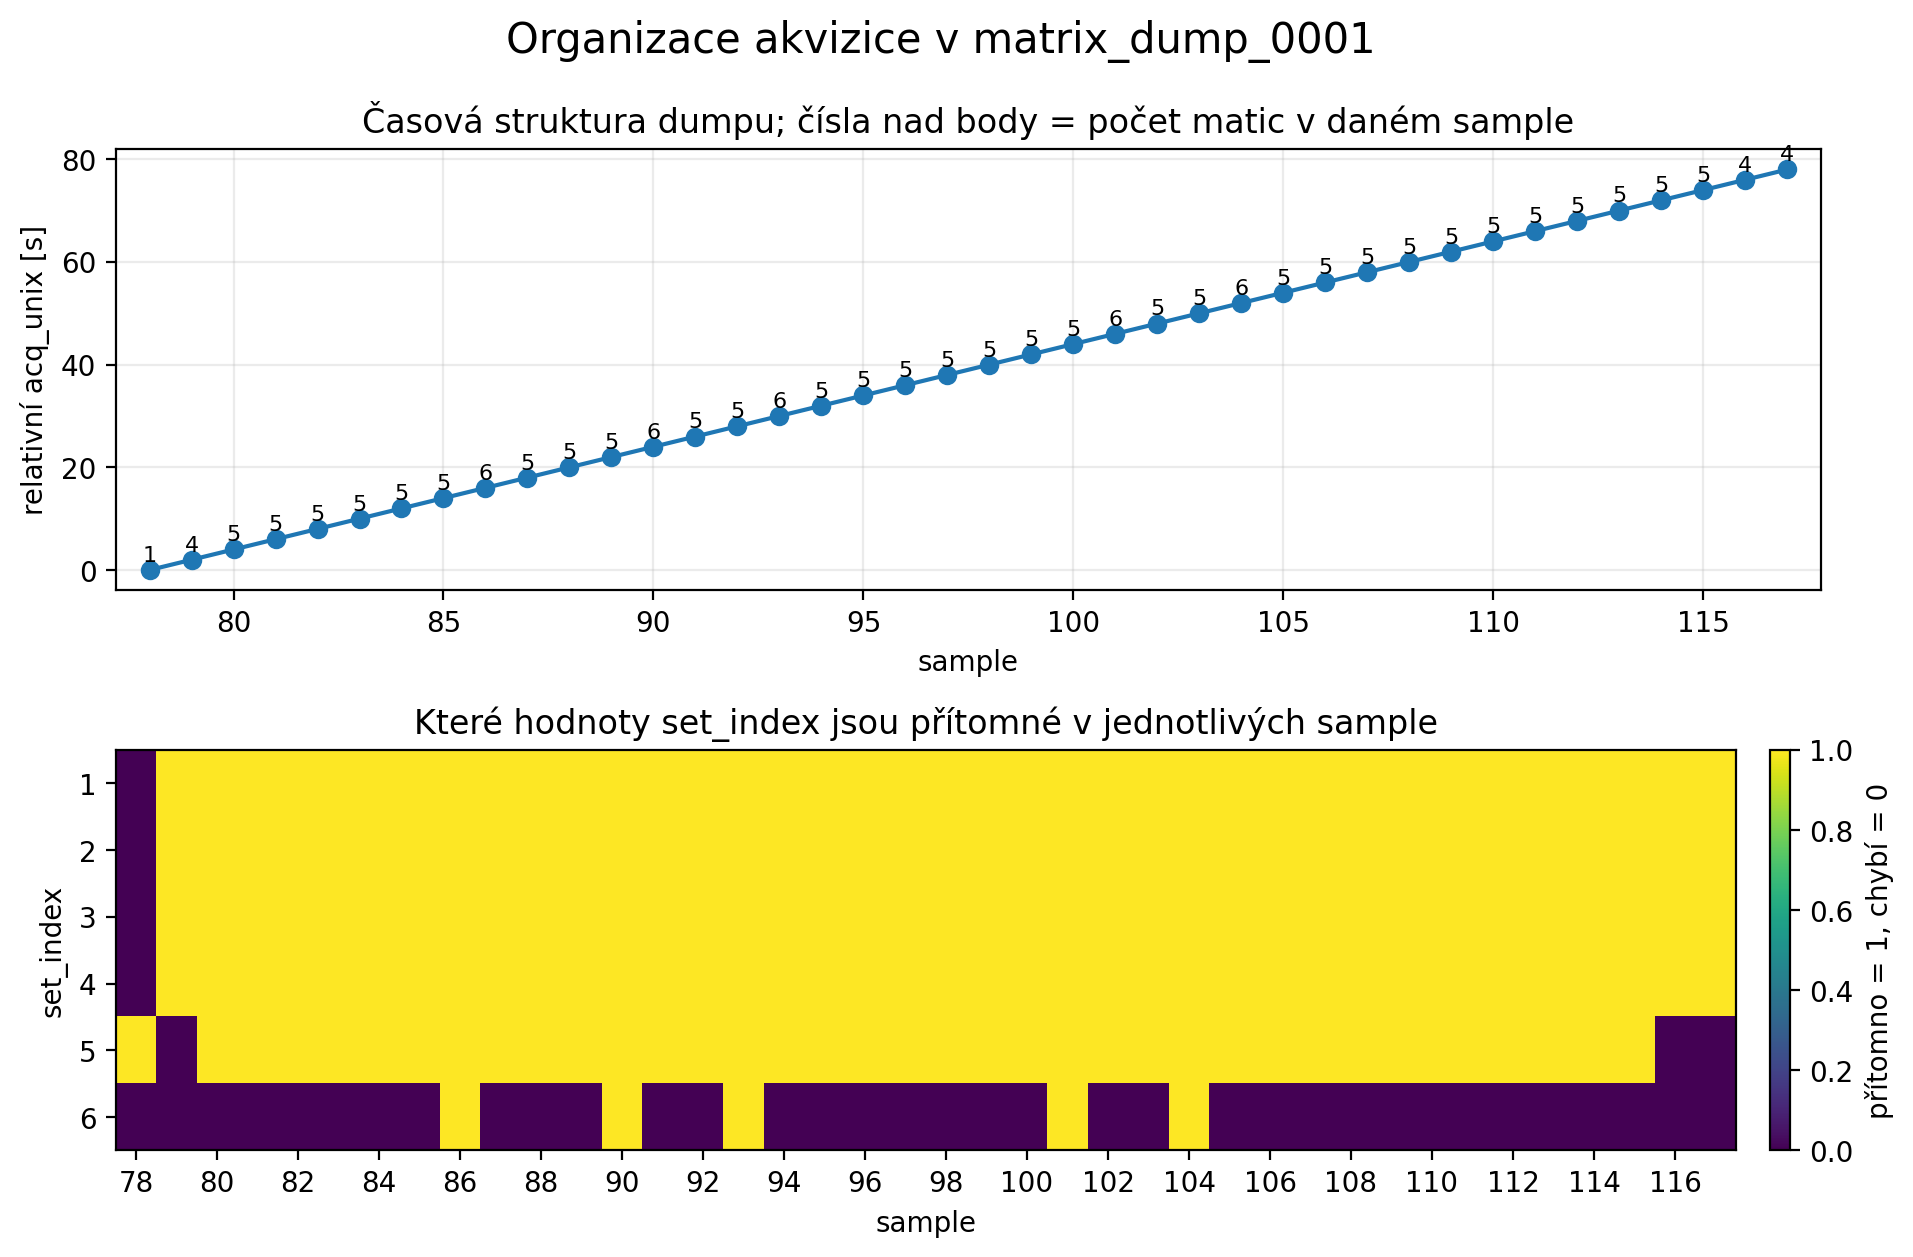
\includegraphics[width=\textwidth]{assets/temporal_structure.png}
    \caption{Časová organizace dumpu. Nahoře je vidět lineární vztah mezi \texttt{sample} a relativním časem \texttt{acq\_unix}; čísla nad body udávají, kolik matic se v daném \texttt{sample} nachází. Dole je přítomnost jednotlivých \texttt{set\_index} v čase.}
    \label{fig:temporal-structure}
\end{figure}

Praktický důsledek pro modelování je zásadní: pokud budete chtít využít čas, přirozená struktura dat není ``jedna 2D matice'', ale spíše \emph{časový blok \texttt{sample} obsahující několik paralelních řídkých matic}. To favorizuje multi-view nebo set-based reprezentaci nad prostým sečtením všeho do jedné 2D mapy.

\subsection{Co přesně znamená pixel}

Každá matice má tvar $256\times256$ a je uložená ve sparse formátu. To znamená, že v textu jsou uvedeny pouze nenulové pixely; všechny chybějící souřadnice je třeba interpretovat jako nulovou energii:
\[
M^{(\texttt{sample},\,\texttt{set})}_{x,y} =
\begin{cases}
E_{x,y} > 0, & \text{pokud je pixel } (x,y) \text{ uveden v } \texttt{entries},\\
0, & \text{jinak.}
\end{cases}
\]

Souřadnice \texttt{x} a \texttt{y} jsou celočíselné indexy v rozsahu 0 až 255. Hodnota \texttt{energy} je skalár -- kalibrovaná energie v dané detektorové buňce. Nejde tedy o obraz s více barevnými kanály, ale o fyzikální mapu depozic v pravidelné mřížce. To je z pohledu strojového učení velmi důležité: ``pixel'' zde není vizuální texel, ale \textbf{detektorový hit nebo buněčná depozice}.

Napříč celým dumpem je 187\,771 aktivních pixelů. Energie v aktivním pixelu je vždy kladná; minimum je 2.52, medián 18.87, 99. percentil 459.55 a maximum 2246.59. Souřadnice se v rámci jedné matice nikdy neduplikují, takže každý záznam je skutečně standardní řídká matice, nikoli multiset hitů na stejné buňce. Typický snímek je tvořen směsí izolovaných bodových depozit, krátkých lineárních stop a malých kompaktních shluků. To je přesně ten typ morfologie, kde je rozumné kombinovat lokaci, tvar, energii a případně čas.

\subsection{Statistický profil dumpu}

Z dodaného \texttt{matrix\_dump\_0001.zip} jsem automaticky naparsoval 198 záznamů. Základní statistiky shrnuje tabulka~\ref{tab:dump-stats}. Většina matic je velmi řídká; medián nenulových prvků je 1154.5 z celkových 65536 buněk, což odpovídá zhruba \SI{1.76}{\percent} aktivních pixelů. Průměrná obsazenost přes celý dump je \SI{1.45}{\percent}, tedy přibližně \SI{98.55}{\percent} obrazu je nulových. To je hlavní argument proti slepému používání velkých hustých CNN na celé snímky.

\begin{table}[H]
\centering
\caption{Shrnutí naparsovaného dumpu \texttt{matrix\_dump\_0001.zip}.}
\label{tab:dump-stats}
\begin{tabularx}{\textwidth}{@{}l r@{}}
\toprule
\textbf{Velikost / statistika} & \textbf{Hodnota} \\
\midrule
Počet matic & 198 \\
Počet unikátních \texttt{sample} & 40 \\
Rozsah \texttt{sample} & 78 až 117 \\
Krok indexu \texttt{sample} & 1 \\
Krok \texttt{acq\_unix} mezi sousedními \texttt{sample} & 2 s \\
Pokrytá délka sekvence podle \texttt{acq\_unix} & 78 s \\
Rozměr matice & $256\times256$ \\
Matice na \texttt{sample} (min / medián / průměr / max) & 1 / 5 / 4.95 / 6 \\
Typické hodnoty \texttt{set\_index} & 1 až 5; hodnota 6 jen v pěti blocích \\
Počet nenulových buněk (min / medián / průměr / max) & 3 / 1154.5 / 948.3 / 1736 \\
Celkový počet nenulových buněk v dumpu & 187771 \\
Průměrná obsazenost & \SI{1.45}{\percent} \\
Medián obsazenosti & \SI{1.76}{\percent} \\
Počet matic s \texttt{nnz} $< 100$ & 34 \\
Součet energie na matici (min / medián / max) & 71.9 / 74687.3 / 117503.0 \\
Energie v aktivním pixelu (min / medián / q99 / max) & 2.52 / 18.87 / 459.55 / 2246.59 \\
\texttt{hw\_t0\_ns} (min / medián / max) & 1634 / 1008425 / 4243614 \\
\texttt{hw\_t\_proc\_ns} (min / medián / max) & 206289331 / 249274857 / 249997164 \\
\bottomrule
\end{tabularx}
\end{table}

\begin{figure}[H]
    \centering
    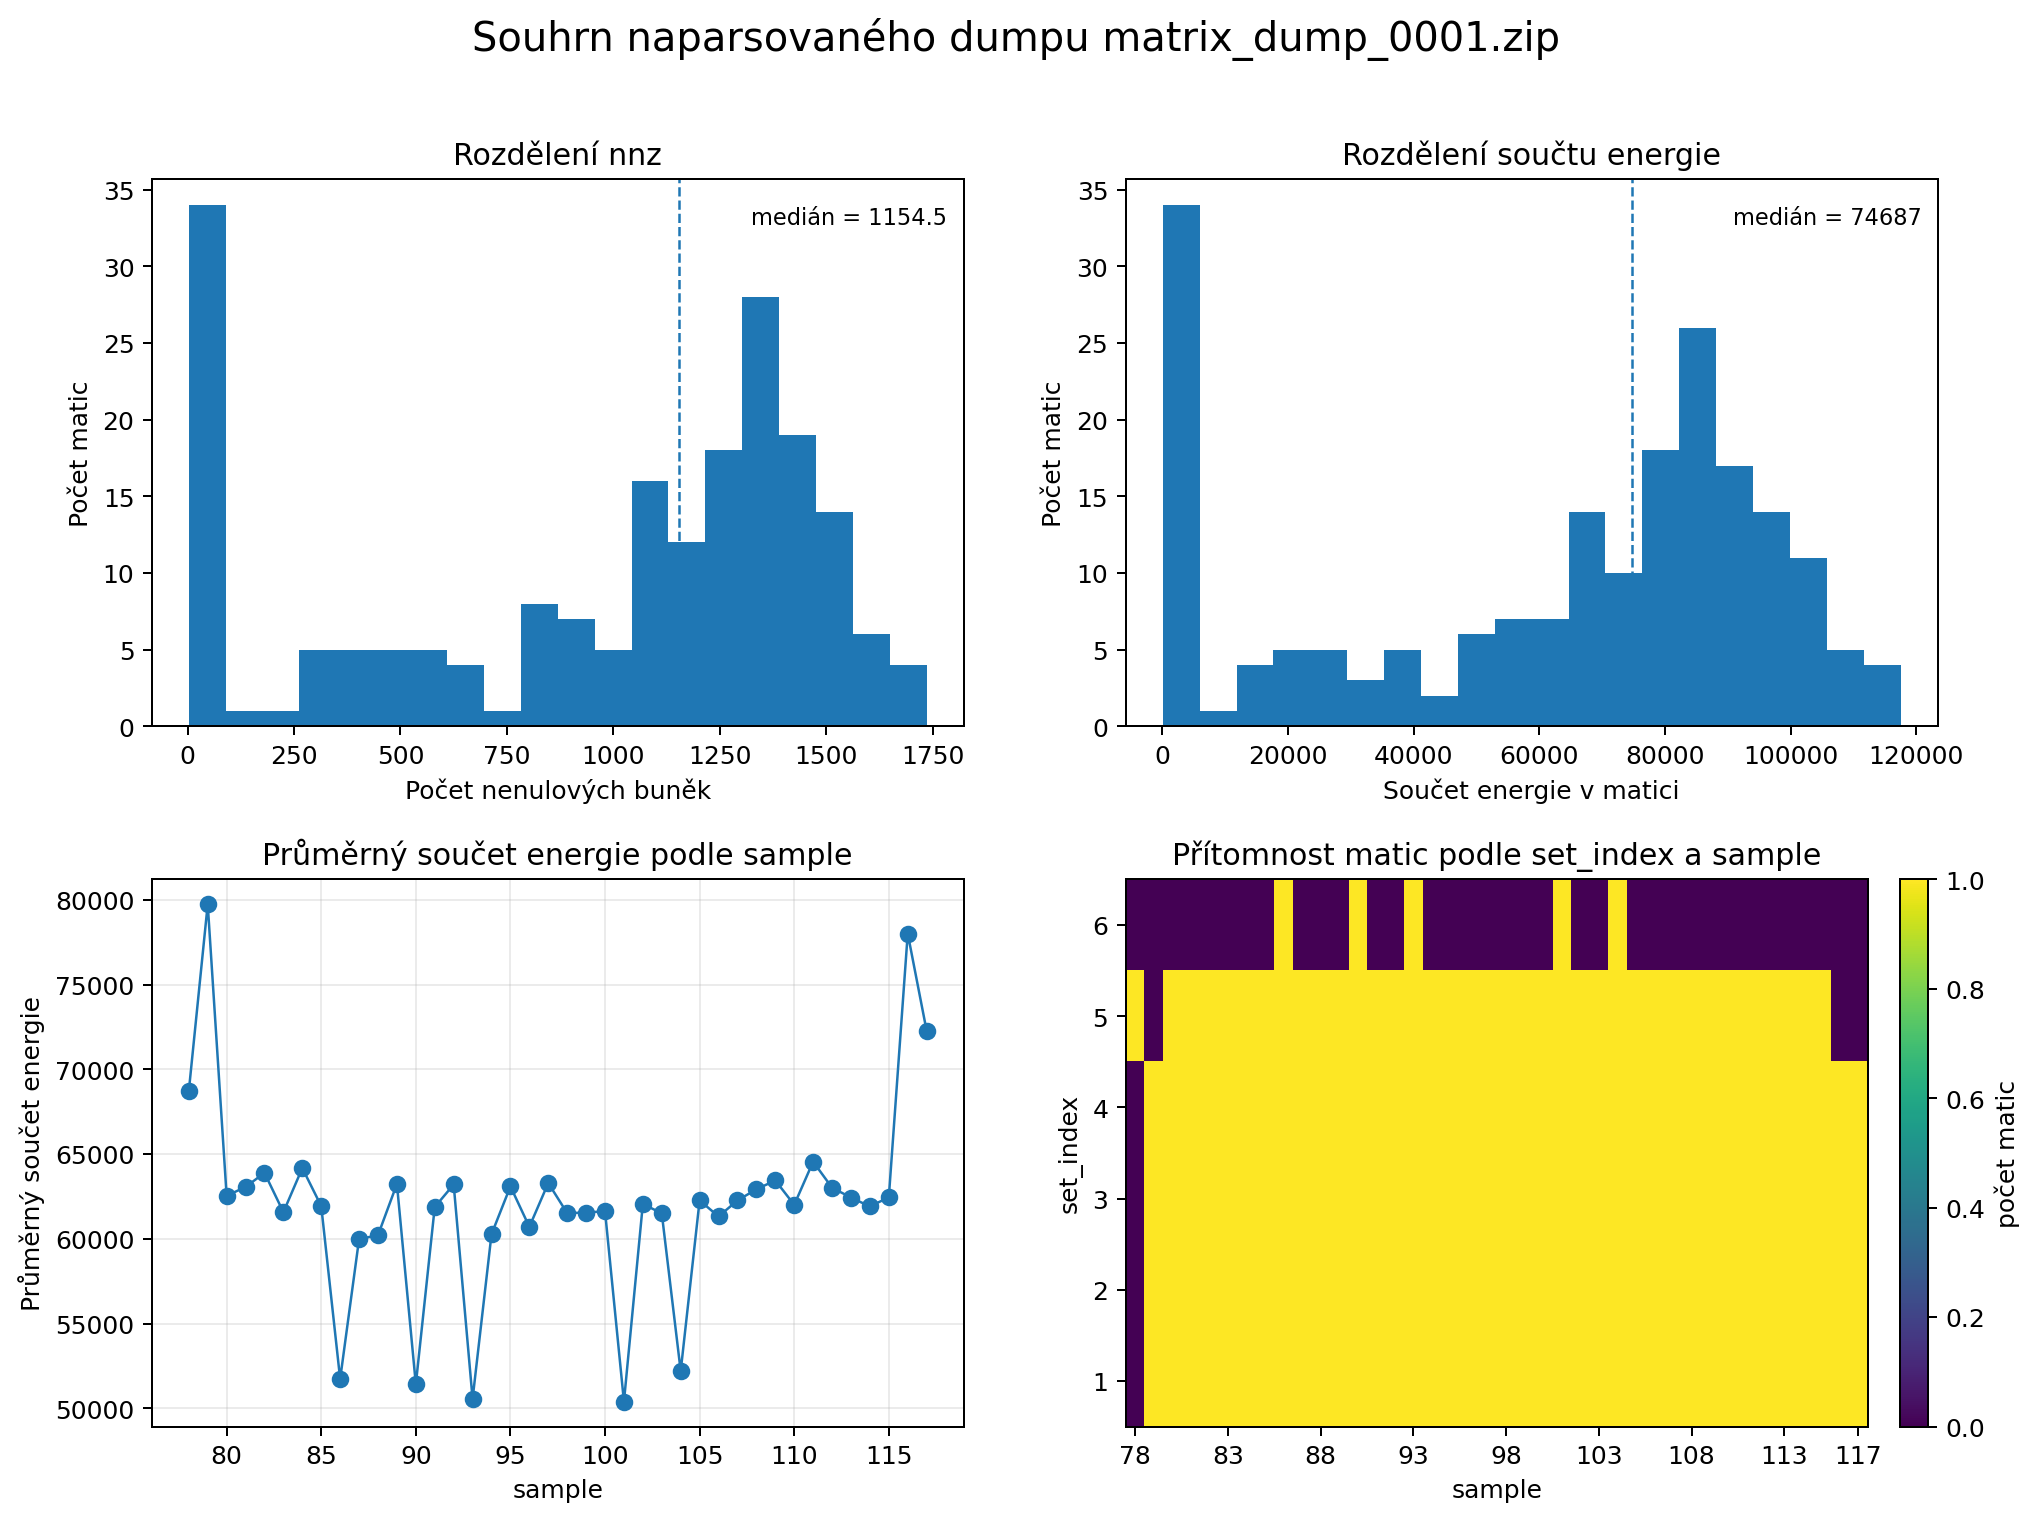
\includegraphics[width=\textwidth]{assets/dataset_summary.png}
    \caption{Levá část: rozdělení počtu nenulových pixelů na matici. Pravá část: průměrný součet energie pro jednotlivé hodnoty \texttt{sample}. Je vidět, že dump obsahuje jak téměř prázdné rámce, tak hustší snímky s velkým počtem menších depozit.}
    \label{fig:dataset-summary}
\end{figure}

\begin{figure}[H]
    \centering
    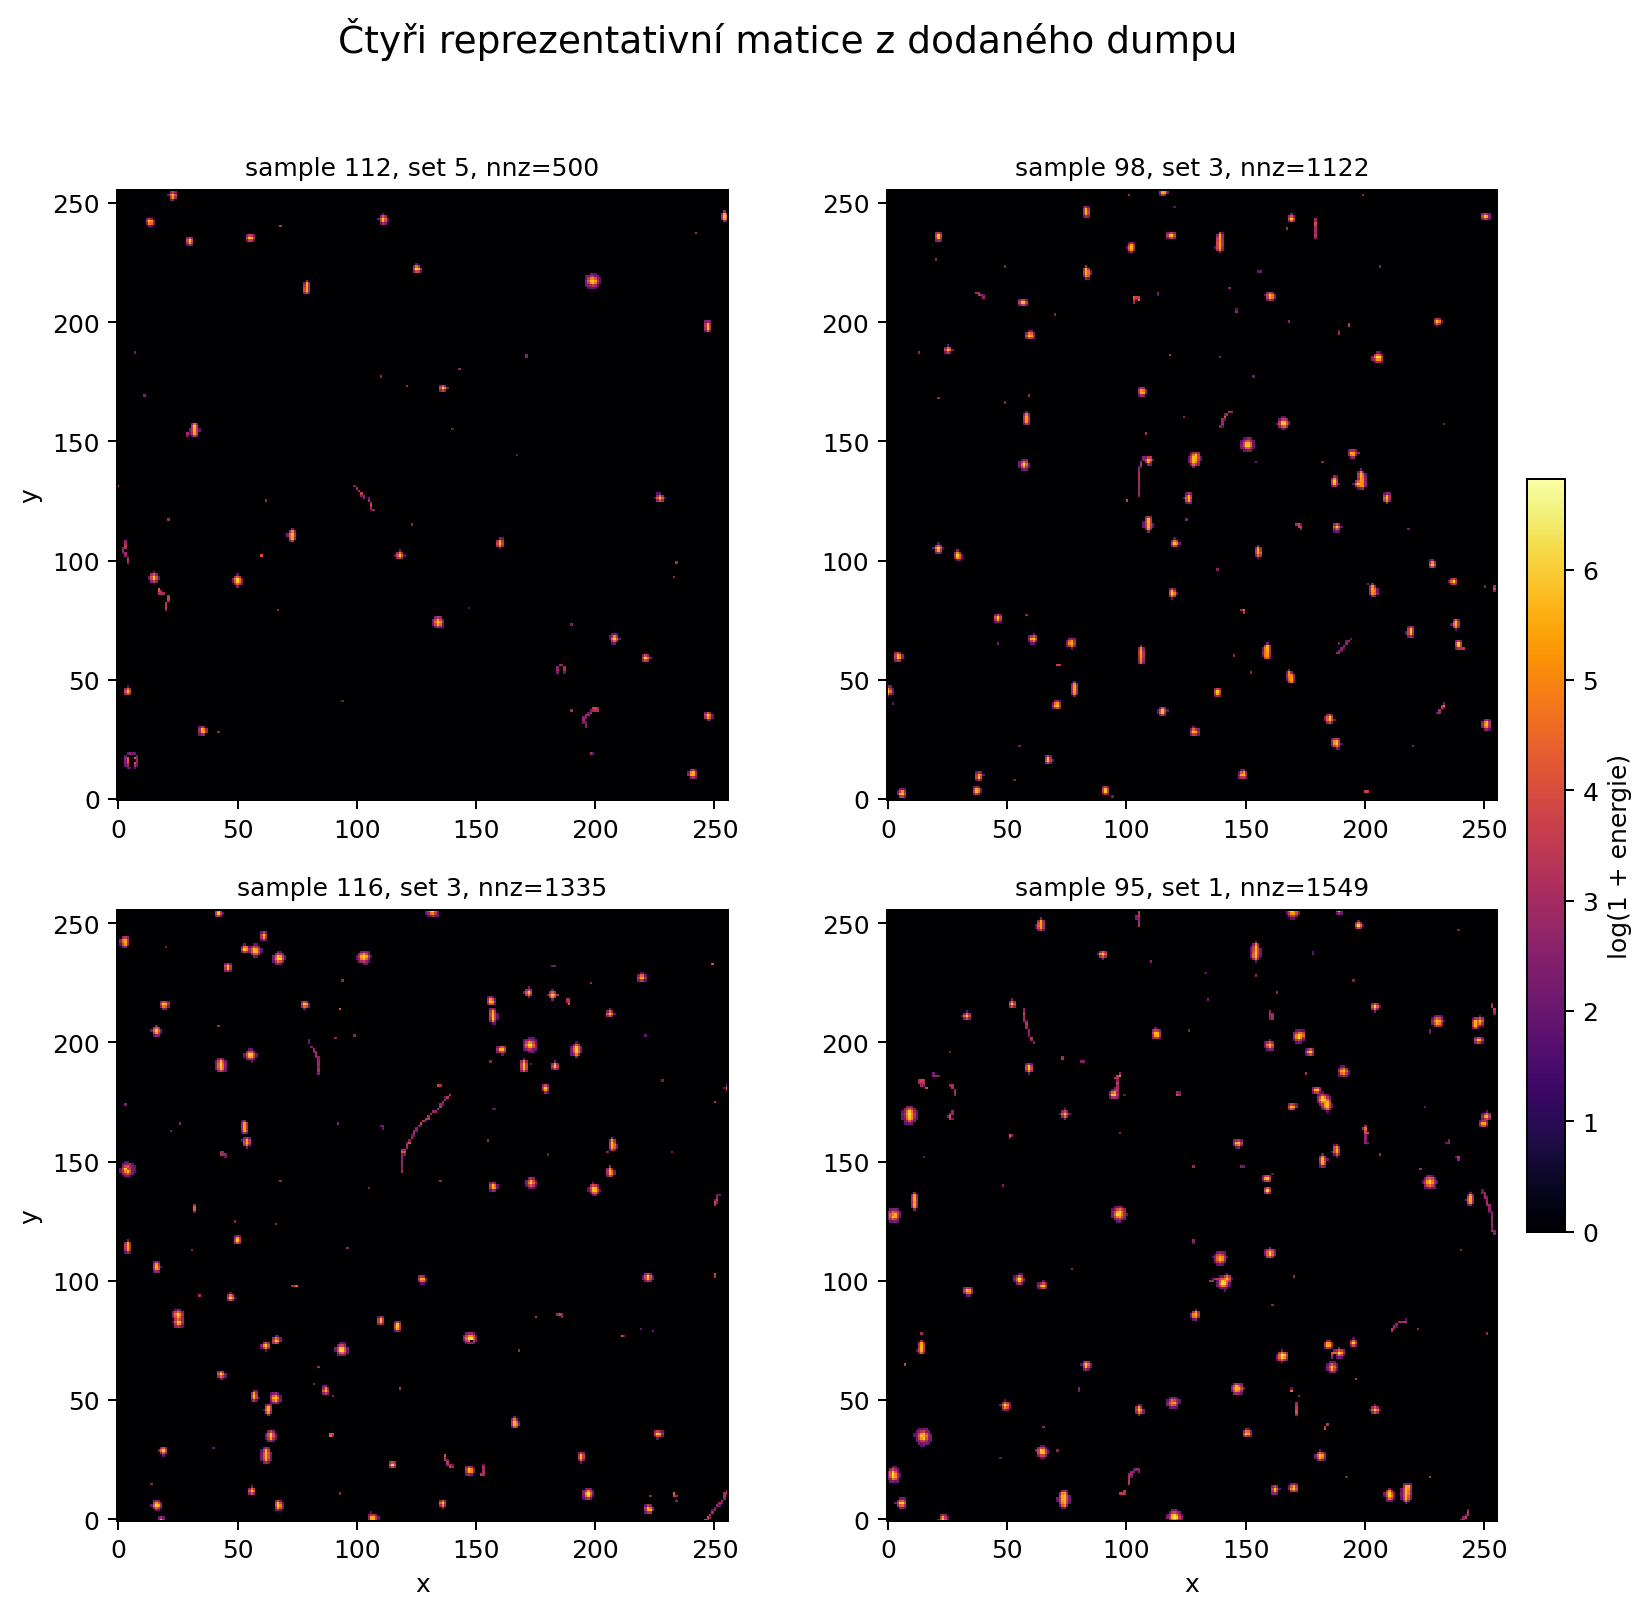
\includegraphics[width=\textwidth]{assets/examples_from_dump.png}
    \caption{Čtyři ukázkové matice přímo z dodaného dumpu. Z hlediska morfologie je patrná směs izolovaných bodových depozit, krátkých lineárních stop a lokálně kompaktních shluků s výrazným energetickým maximem.}
    \label{fig:examples-dump}
\end{figure}

\subsection{Co ukazují přiložené screenshoty}

Screenshoty raw/DBSCAN jsou užitečné, protože zviditelňují současný pracovní postup i jeho limity. Například sjednocení rámců 89--96 obsahuje 8808 hitů a po DBSCANu dává 525 clusterů a 357 bodů označených jako šum. Jednotlivé snímky 67 a 176 mají kolem 1000--1300 hitů a zhruba 60--70 clusterů. Z obrazů je zřejmé, že se v datech vyskytují jak téměř bodové depozice, tak krátké lineární stopy a malé překryvy.

\begin{figure}[p]
    \centering
    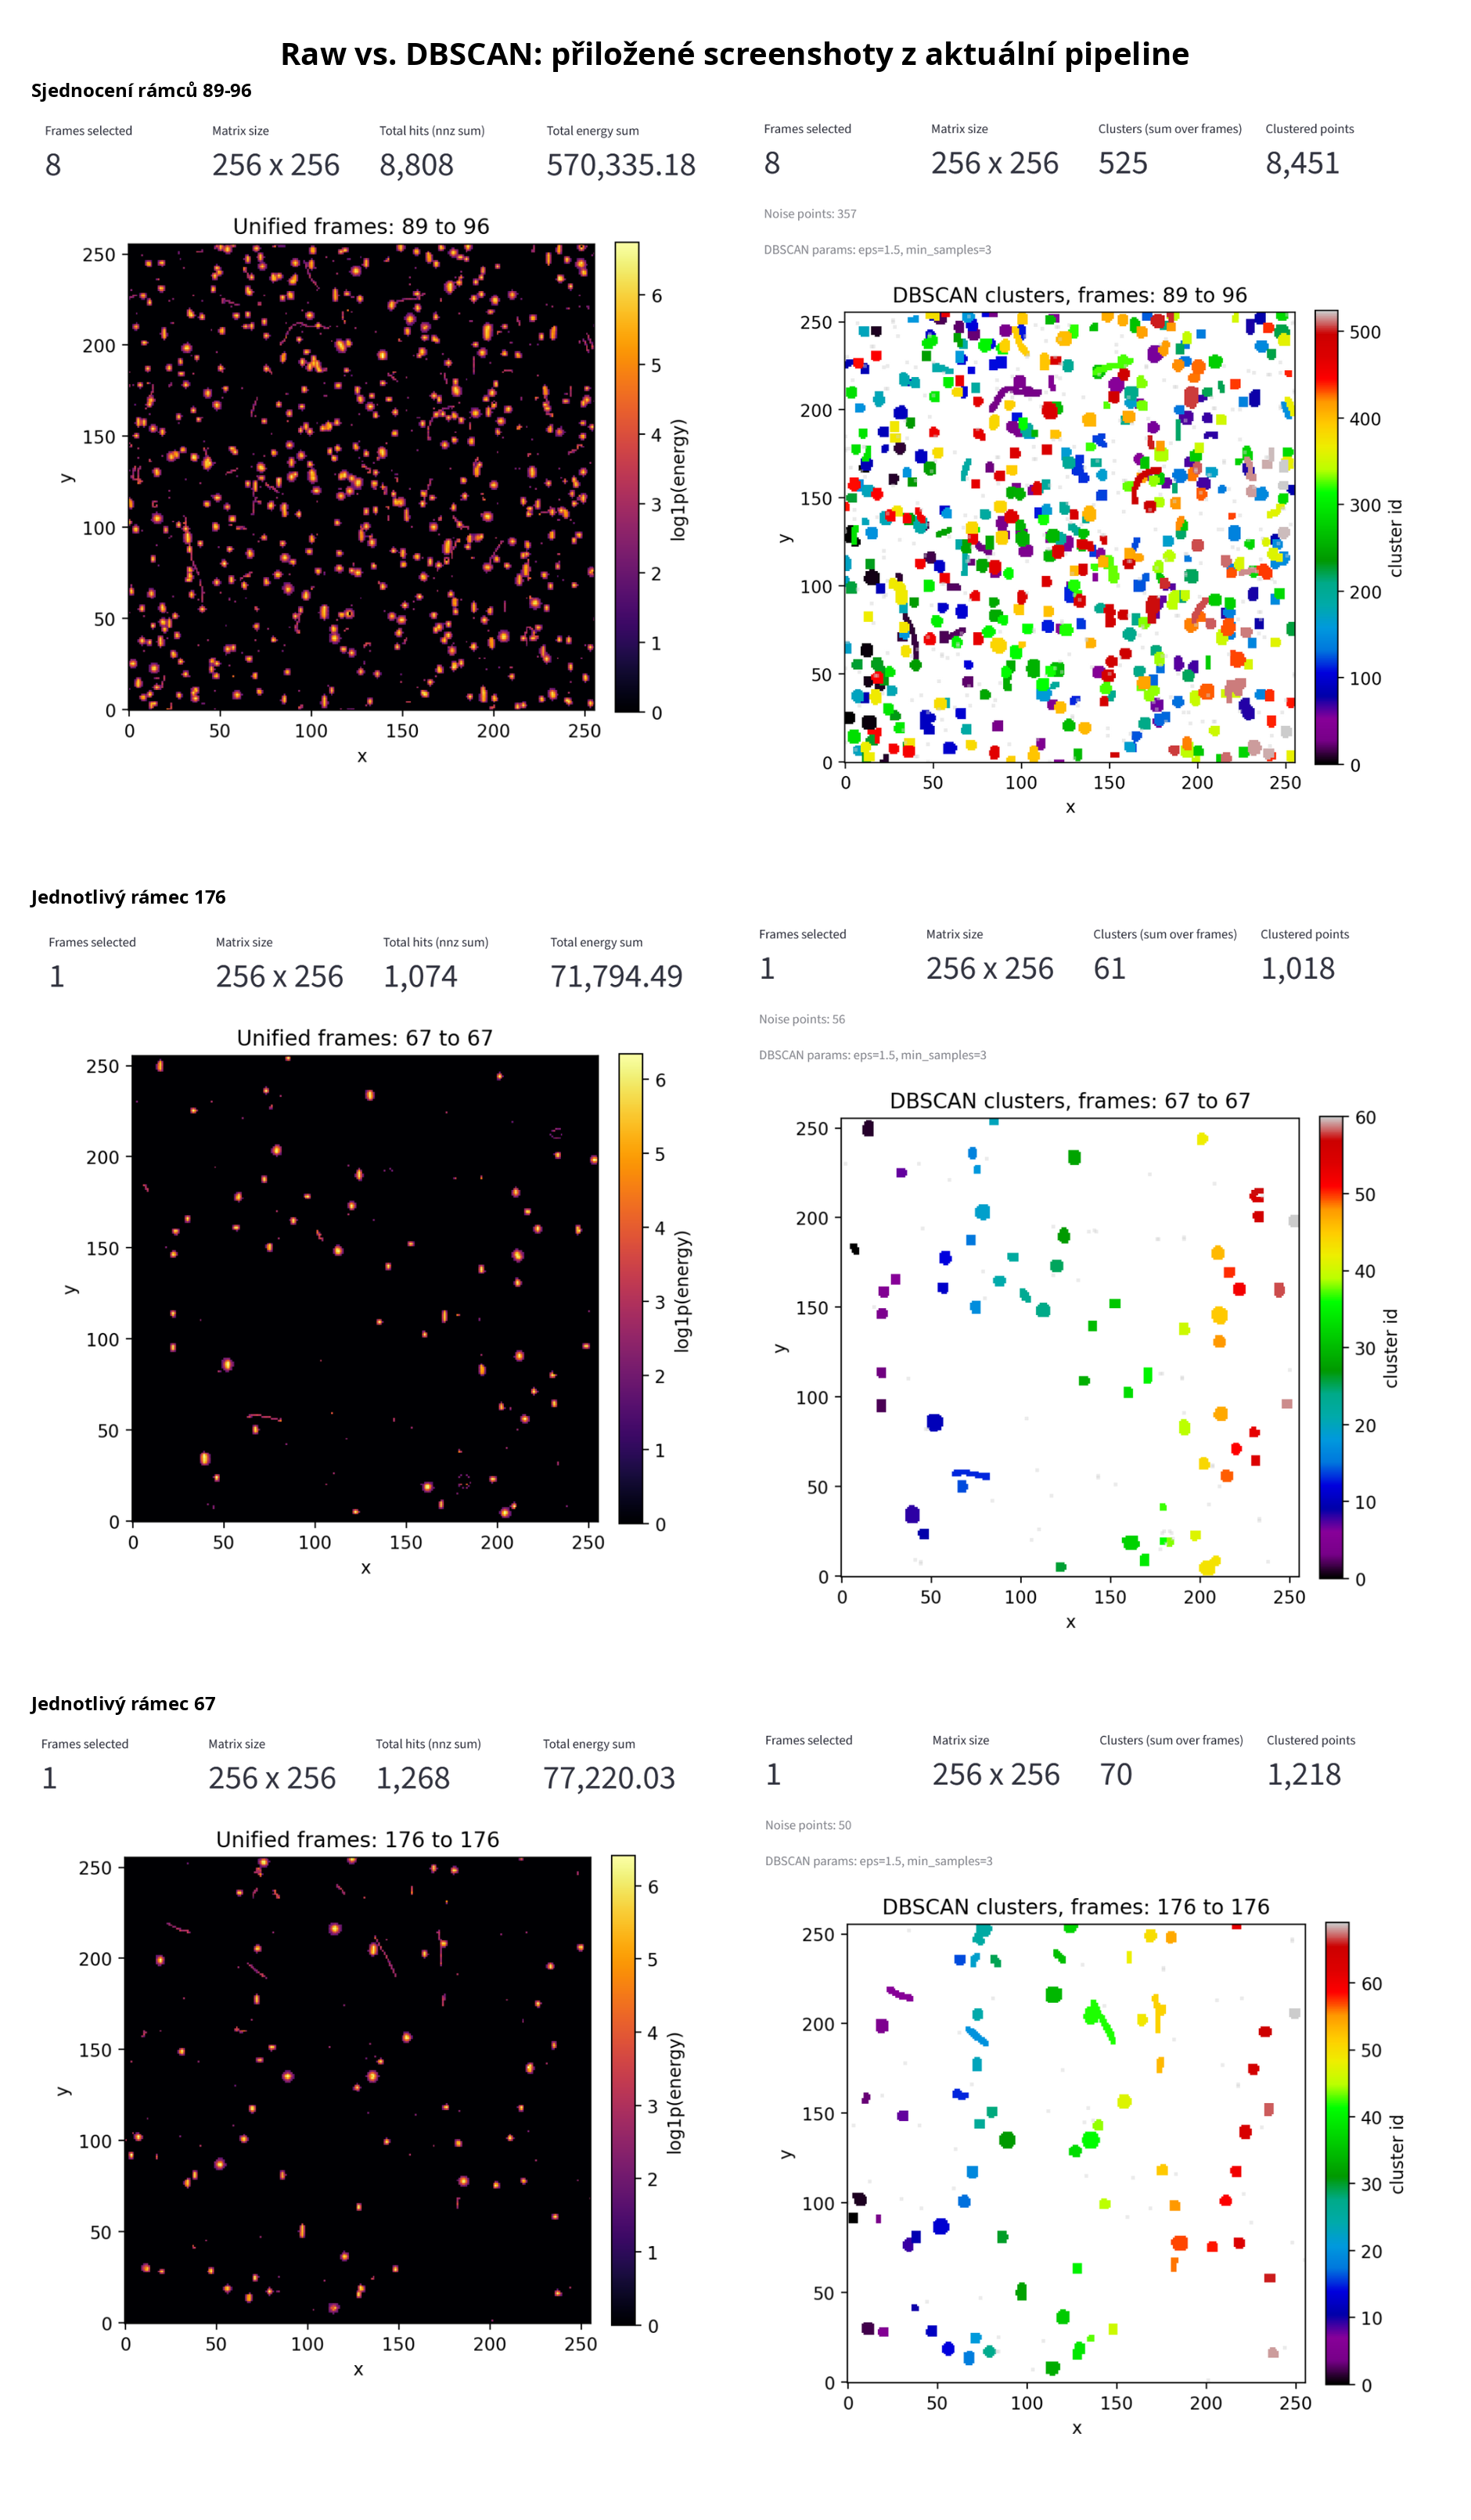
\includegraphics[width=\textwidth,height=0.91\textheight,keepaspectratio]{assets/dbscan_examples_collage.png}
    \caption{Přiložené screenshoty raw zobrazení a výstupu DBSCANu. Tyto obrázky dobře ilustrují, že současný klastrovací postup už v praxi funguje jako detektor kandidátů, ale zároveň je závislý na globální volbě \texttt{eps} a \texttt{min\_samples} a ignoruje většinu kontextu, který by šel neuronově vytěžit.}
    \label{fig:dbscan-collage}
\end{figure}

\clearpage

\section{Co z dat vlastně chceme vyrobit / určit}
\label{sec:targets}

Samotný dump ještě neobsahuje ``klasifikaci částic''; obsahuje pouze měřená data. Aby byl projekt dobře definovaný, je potřeba oddělit několik vrstev výstupu. Jinak snadno vznikne zmatek mezi tím, co je přímo měřená depozice v pixelu, co je rekonstruovaný cluster a co je už fyzikální interpretace. U těchto dat je velmi užitečné uvažovat následující posloupnost:

\begin{enumerate}
    \item \textbf{P1 -- čištění a hit filtering:} rozhodnout, které aktivní pixely jsou fyzikálně relevantní signál a které jsou šum nebo artefakt.
    \item \textbf{P2 -- clustering / instance segmentace:} určit, které pixely patří k sobě a tvoří jednu depozici, stopu nebo spršku.
    \item \textbf{P3 -- klasifikace objektu:} každému clusteru nebo stopě přiřadit morfologickou nebo fyzikální třídu a důvěru.
    \item \textbf{P4 -- asociace přes čas nebo více pohledů:} rozhodnout, které objekty v různých \texttt{set\_index} nebo sousedních \texttt{sample} patří k témuž fyzikálnímu objektu.
    \item \textbf{P5 -- sample/event-level souhrn:} ze všech výše uvedených kroků vytvořit počty, spektra, rate estimate, trigger nebo anomální skóre.
\end{enumerate}

V současném workflow, které už používá DBSCAN, je implicitně řešen hlavně krok P2. Jakmile se řekne ``klasifikace částic'', je ale potřeba doplnit i P3 a ujasnit, zda výstupem má být \emph{morfologická třída} (např. bodový deposit, krátká stopa, dlouhá stopa, kompaktní sprška, překryv, šum) nebo \emph{fyzikální druh částice}. To jsou dvě odlišné úlohy; druhá z nich obvykle vyžaduje víc kontextu než jen jednu 2D projekci.

\begin{table}[H]
\centering
\caption{Jaké produkty lze z dat rozumně vyrábět a co k nim potřebujete.}
\label{tab:target-products}
\small
\begin{tabularx}{\textwidth}{@{}>{\raggedright\arraybackslash}p{0.10\textwidth} >{\raggedright\arraybackslash}p{0.18\textwidth} Y >{\raggedright\arraybackslash}p{0.24\textwidth}@{}}
\toprule
\textbf{Krok} & \textbf{Jednotka} & \textbf{Co je přímý výstup} & \textbf{Jaká pravda / anotace je potřeba} \\
\midrule
P1 & aktivní pixel / hit & signal vs. šum, případně váha nebo maska & hit-level labely, simulace, nebo konzervativní heuristiky \\
P2 & množina hitů v rámci jednoho \texttt{sample} a \texttt{set\_index} & cluster ID pro každý hit, případně instance maska & instance-level truth nebo kvalitní baseline clustering \\
P3 & cluster / stopa / sprška & třída objektu + confidence + případně regrese energie a polohy & cluster-level třídy; pro fyzikální PID typicky simulace nebo ruční anotace \\
P4 & dvojice či sada objektů napříč rámci & linky mezi view nebo časem, tracklet, sjednocený objekt & identita objektu přes více pohledů či časové bloky \\
P5 & celý \texttt{sample} nebo celý běh & počty objektů, energetická spektra, trigger score, anomaly score & event-level labely nebo unsupervised cíl \\
\bottomrule
\end{tabularx}
\end{table}
\normalsize

\subsection{Doporučený první cíl projektu}

Pro přiložený dump a současné screenshoty je nejrozumnější první praktická formulace úlohy:
\begin{center}
\emph{aktivní pixely $\rightarrow$ cluster candidate (P2) $\rightarrow$ cluster-level klasifikace a confidence (P3).}
\end{center}

Tato formulace je silná z několika důvodů. Za prvé navazuje přímo na to, co už dnes děláte pomocí DBSCANu. Za druhé nevyžaduje hned řešit plně end-to-end rekonstrukci na hit-level pravdě. Za třetí vám dává použitelný produkt už v první etapě: pro každý cluster dostanete nejen jeho hranici nebo identitu, ale i \textbf{třídu, důvěru a sadu fyzikálně smysluplných atributů}. A konečně je to výstup, který lze později rozšířit na P4 a P5 bez toho, aby se musela vyhodit celá pipeline.

\begin{tcolorbox}[colback=AccentLight,colframe=Accent,title=\textbf{Doporučený první deliverable}]
Pro každý objekt vracet minimálně: \texttt{sample}, \texttt{set\_index}, \texttt{cluster\_id}, seznam nebo masku hitů, celkovou energii, velikost, excentricitu, odhadovanou třídu, confidence a případně flag ``nejistý / out-of-distribution''. Tento formát je vhodný jak pro online analýzu, tak pro pozdější fyzikální validaci.
\end{tcolorbox}

\subsection{Morfologická třída versus fyzikální druh částice}

Z aktuálního dumpu samotného nelze přímo vyčíst ground truth fyzikálního druhu částice. Proto doporučuji rozlišit dva režimy:

\begin{itemize}
    \item \textbf{Morfologická klasifikace.} Síť se učí rozpoznávat tvarové a energetické typy objektů: izolovaný bodový deposit, krátká stopa, dlouhá stopa, sprška, překryv, šum. To je realistické i bez plné simulace a často je to nejlepší první mezikrok.
    \item \textbf{Fyzikální PID.} Síť se učí mapovat rekonstruovaný objekt na fyzikální hypotézu částice. To je silnější cíl, ale typicky vyžaduje simulaci, beam metadata, geometrii detektoru nebo další detektorové kanály.
\end{itemize}

Jinými slovy: pokud v této fázi nemáte spolehlivou externí pravdu, je bezpečnější začít morfologickou taxonomií a teprve potom ji mapovat na fyzikální interpretaci. Tím se výrazně sníží riziko, že bude model přeučený na heuristické ``částicové'' štítky, které ve skutečnosti popisují jen tvar v 2D projekci.

\subsection{Odkud vezmou štítky pravdu}

Samotný dodaný dump fyzikální třídy částic neobsahuje. Máte tedy v zásadě čtyři možnosti:

\begin{itemize}
    \item \textbf{Simulace s Monte Carlo truth.} To je pro supervised trénink nejlepší varianta a prakticky nutnost, pokud chcete jít cestou object condensation nebo hit-level segmentace.
    \item \textbf{Ruční anotace malého počtu clusterů.} Vhodné pro pilotní cluster classifier a pro definici morfologických tříd.
    \item \textbf{Vysokodůvěrné heuristiky.} Například extrémně kompaktní, izolované clustery jako pseudo-štítky pro ``bodový deposit'', dlouhé lineární útvary pro ``stopu'' apod. To je užitečné pro bootstrap, ale ne jako finální ground truth.
    \item \textbf{Samoučené předtrénování.} Nejprve se síť naučí reprezentaci bez štítků, teprve potom se malý klasifikační head doučí na omezené anotaci \citep{young2025polarmae,young2025panda,park2025fm4npp}.
\end{itemize}

Velmi důležité je i to, že některé částice nemusí být z jedné 2D matice spolehlivě rozlišitelné jen podle tvaru. Pokud chcete jít až na fyzikální identifikaci typu částice, je výhodné přidat čas, více pohledů a případně další detektorové kontexty. Pokud taková informace k dispozici není, doporučuji zavést nejprve morfologické třídy a teprve následně je mapovat na fyzikální hypotézy.


\section{Proč samotný DBSCAN nestačí, ale je stále užitečný}

V terminologii sekce~\ref{sec:targets} řeší DBSCAN především krok P2, tedy clustering nebo instance segmentaci aktivních hitů. Sám o sobě ale neřeší P3, tj. klasifikaci objektu, a už vůbec ne P4, tedy asociaci přes čas nebo více paralelních pohledů. Jako současný baseline je přesto rozumný: umí najít clustery libovolného tvaru, dobře pracuje s izolovanými body a je interpretovatelný \citep{ester1996dbscan}. V kontextu vašich dat má ale několik strukturálních limitů:

\begin{itemize}
    \item \textbf{Globální hustotní předpoklad.} Jedna volba \texttt{eps} a \texttt{min\_samples} musí fungovat pro bodové depozity, krátké stopy i hustší shluky.
    \item \textbf{Energie a čas nejsou přirozeně součástí modelu.} Lze je přidat do metriky nebo následné klasifikace, ale DBSCAN se je sám nenaučí využívat adaptivně.
    \item \textbf{Překryvy a proměnlivá lokální hustota.} Tam DBSCAN typicky mergeuje nebo oversplittuje.
    \item \textbf{Agregace v čase.} Pokud se rámce jen sečtou, ztratí se pořadí a do jednoho obrazu se promítnou procesy s různou časovou strukturou.
\end{itemize}

To ale neznamená, že je třeba DBSCAN zahodit. Naopak:

\begin{itemize}
    \item Je vhodný jako \textbf{interpretable baseline}.
    \item Je vhodný jako \textbf{region proposal generator} pro klasifikaci clusterů.
    \item Je vhodný jako \textbf{zdroj pseudo-štítků} nebo vysokodůvěrných negativních příkladů.
    \item Pokud chcete dočasně využít i čas, lze jako mezikrok vyzkoušet prostorově-časový variantní baseline typu ST-DBSCAN \citep{birant2007stdbscan}.
\end{itemize}

Dobré praktické pravidlo je tedy: \textbf{DBSCAN ponechat jako rychlý bootstrap, ale nebrat jej jako konečný rekonstrukční model.}

\section{Možné neuronové přístupy}

\subsection{Nejrychlejší baseline: DBSCAN + klasifikátor clusterů}

Toto je nejpřímější implementace pipeline P2 $\rightarrow$ P3 a zároveň nejrychlejší cesta k prvnímu použitelnému systému. Prakticky může vypadat takto:

\begin{enumerate}
    \item raw matice $\rightarrow$ základní thresholding / denoising,
    \item DBSCAN $\rightarrow$ kandidátní clustery,
    \item pro každý cluster vytvořit ořez (\emph{crop}) nebo seznam hitů,
    \item klasifikátor vrátí třídu clusteru a případně jeho důvěru.
\end{enumerate}

Takový klasifikátor může mít dvě větve:
\begin{itemize}
    \item \textbf{obrazovou větev:} malý CNN nad ořezem clusteru, typicky $32\times32$ až $64\times64$,
    \item \textbf{tabulkovou větev:} skalární rysy jako celková energie, maximum, excentricita, délka skeletonu, počet hitů, momenty tvaru, \texttt{hw\_t0\_ns}, \texttt{hw\_t\_proc\_ns}, \texttt{set\_index}.
\end{itemize}

Výhoda je zřejmá: jde o rychlý, levný a velmi interpretovatelný systém. Nevýhoda je, že úspěch je limitován kvalitou DBSCAN clusterů. Jakmile se cluster rozdělí nebo slije špatně, klasifikátor to už typicky nezachrání.

\subsection{Sparse CNN a U-Net nad celým snímkem}

Jestliže chcete zůstat u mřížkové reprezentace, ale nechcete plýtvat výpočtem na nulových pixelech, dává smysl sparse konvoluční síť. Základní teoretický i praktický rámec vytvořily \emph{submanifold sparse convolutions} a knihovna Minkowski Engine \citep{graham2017submanifold,choy2019minkowski}. V HEP a neutrinové fyzice jsou sparse U-Net a sparse ResNet běžným základem rekonstrukčních řetězců \citep{drielsma2021spine}.

Tento směr je vhodný zejména tehdy, pokud:
\begin{itemize}
    \item geometrie je opravdu pravidelná mřížka a lokální sousedství má fyzikální smysl,
    \item chcete dělat hit-level segmentaci nebo denoising,
    \item chcete zachovat celosnímkový kontext bez explicitního DBSCAN kroku.
\end{itemize}

Váš případ tomu odpovídá částečně. Pro jeden samotný snímek $256\times256$ není husté CNN ještě výpočetně nemožné. Jakmile ale budete chtít přidat více rámců, více pohledů nebo dělat plně end-to-end segmentaci, sparse CNN začne být výrazně výhodnější.

\subsection{Point-set a grafové modely}

Pro vaše data je to podle mého názoru \textbf{nejlepší střednědobý kompromis}. Nenulové body se přirozeně zapíší jako množina
\[
\mathcal{H} = \{(x_i,y_i,E_i,t_i,\Delta t_i,s_i)\}_{i=1}^{N},
\]
kde $s_i$ může nést například \texttt{set\_index}. Síť pak pracuje jen nad aktivními hity. Tento směr je velmi blízký tomu, co dnes dělají moderní GNN v rekonstrukci částic \citep{qasim2019gravnet,shlomi2020gnn,thais2022gnnreview}.

Prakticky lze použít například:
\begin{itemize}
    \item \textbf{GravNet / GarNet} pro učení latentního sousedství přímo z dat \citep{qasim2019gravnet},
    \item \textbf{EdgeConv/ParticleNet-style modely} tam, kde je výhodné dynamicky přebudovávat graf \citep{qu2020particlenet},
    \item \textbf{set/point transformers} tam, kde je klíčové modelovat dlouhodosahové vazby a více pohledů \citep{qu2022part,robles2025pointset}.
\end{itemize}

Hlavní výhody:
\begin{itemize}
    \item reprezentace je \textbf{přímo sparse},
    \item počet hitů se může měnit snímek od snímku,
    \item je přirozené připojit energii, čas i kategorické metadata,
    \item lze modelovat i více pohledů nebo více matic se stejným \texttt{sample}.
\end{itemize}

\subsection{Object condensation: naučené klastrování i klasifikace v jednom kroku}

Pokud je cílem nahradit DBSCAN něčím skutečně silnějším, pak je nejrelevantnější dnešní směr \textbf{object condensation} \citep{kieseler2020objectcondensation}. Síť pro každý hit predikuje:
\begin{itemize}
    \item latentní souřadnice v naučeném prostoru,
    \item ``condensation'' nebo ``beta'' skóre, tj. pravděpodobnost, že hit reprezentuje centrum objektu,
    \item případně i klasifikační a regresní hlavy.
\end{itemize}

Výsledek je velmi atraktivní: v jednom kroku dostanete \emph{instance segmentaci}, tedy přiřazení hitů k objektům, i \emph{klasifikaci objektů}. Tento přístup byl úspěšně nasazen například pro CMS HGCAL \citep{qasim2021hgcal_oc}, velmi recentně pro CLAS12 calorimetr \citep{matousek2025clas12_oc}, a jako součást nejnovějších end-to-end hit-based rekonstrukcí na budoucích urychlovačích \citep{garcia2026hitpf}.

Nevýhoda je jasná: potřebujete hit-level nebo alespoň instance-level ground truth. Bez simulace nebo pečlivé anotace je trénink takového modelu obtížný.

\subsection{Samoučené předtrénování a foundation-model směr}

Když je mnoho neoznačených dat a málo štítků, je stále relevantnější nejprve naučit obecnou reprezentaci detektorových dat a teprve potom jemně doladit malý klasifikátor. Pro sparse detektorová data se v letech 2025--2026 objevilo několik velmi silných prací: masked point modeling v PoLAr-MAE \citep{young2025polarmae}, samodistilační reprezentace Panda \citep{young2025panda}, širší foundation-model linie FM4NPP \citep{park2025fm4npp} a přehledový článek o foundation modelech v HEP \citep{hallin2025foundationreview}.

Tento směr bych pro váš projekt nevzal jako první implementaci, ale jako \textbf{strategii pro druhou fázi}, pokud:
\begin{itemize}
    \item nasbíráte velký archiv neoznačených snímků,
    \item ruční anotace bude drahá,
    \item budete chtít model přenášet mezi běhy, energiemi nebo detektory.
\end{itemize}

\begin{table}[H]
\centering
\caption{Srovnání hlavních rodin modelů pro vaše data.}
\label{tab:method-comparison}
\begin{tabularx}{\textwidth}{@{}l Y Y Y@{}}
\toprule
\textbf{Rodina} & \textbf{Co umí dobře} & \textbf{Nevýhoda} & \textbf{Doporučení pro váš případ} \\
\midrule
DBSCAN + cluster classifier & rychlý baseline, interpretace, málo labelů & závisí na kvalitě DBSCANu & ano, jako první produkční baseline \\
Sparse CNN / U-Net & hit-level segmentace, mřížkový kontext, snadná 3D/4D generalizace & víc engineeringu než jednoduchý CNN crop model & ano, pokud chcete full-frame segmentaci \\
Point-set / GNN & přirozená práce se sparzitou, proměnný počet hitů, snadné přidání času a metadat & potřeba grafu nebo sousednosti & ano, nejsilnější střednědobá volba \\
Object condensation & clustering i klasifikace v jednom kroku, neznámý počet objektů & potřebuje kvalitní truth, složitější trénink & ano, pokud máte simulaci a chcete nahradit DBSCAN \\
SSL / foundation model & šetří labely, dobrý přenos mezi úlohami & vyšší infra náročnost, stále rychle se vyvíjí & až druhá fáze projektu \\
\bottomrule
\end{tabularx}
\end{table}

\section{Jak bych s tím prakticky postupoval}

\subsection{Doporučená reprezentace vstupu}

U každého aktivního hitu bych vytvářel minimálně tyto rysy:
\[
\vect{h}_i = \left[
\frac{x_i}{255},
\frac{y_i}{255},
\log(1+E_i),
\frac{E_i}{\sum_j E_j + \varepsilon},
\texttt{set\_index},
\tilde{t}_0,
\widetilde{\Delta t}
\right].
\]

Zde $\tilde{t}_0$ a $\widetilde{\Delta t}$ jsou normalizované verze \texttt{hw\_t0\_ns} a \texttt{hw\_t\_proc\_ns}. Pokud budete slučovat více rámců, doporučuji \textbf{nepoužívat pouhý součet}, ale přidat:
\begin{itemize}
    \item \textbf{index rámce} jako další diskrétní nebo spojitý rys,
    \item nebo vytvořit 3D sparse tensor $(x,y,k)$, kde $k$ je index rámce,
    \item nebo pracovat se sjednocenou množinou hitů a nechat síť rozhodnout, co je časově související.
\end{itemize}

Součet přes čas je vhodný jen jako baseline. Jakmile čas zahodíte, síť už nikdy nezjistí, zda dva podobné depozity vznikly současně nebo s posunem v rámci intervalu.

\subsection{Referenční architektura, kterou bych stavěl jako první}

S ohledem na definici úlohy v sekci~\ref{sec:targets} bych paralelně stavěl dva modely, které cílí na odlišnou úroveň problému:

\paragraph{Model A: DBSCAN + point-set classifier (pipeline P2 $\rightarrow$ P3).}
\begin{enumerate}
    \item DBSCAN vytvoří kandidátní clustery.
    \item Z každého clusteru se vezmou všechny hity a jejich znaky.
    \item Nad hity clusteru se postaví malý $k$NN graf (např. $k=12$ až 16).
    \item Backbone: 4 až 6 bloků typu GravNet nebo EdgeConv, šířky 64--128 kanálů.
    \item Global pooling + klasifikační hlava.
    \item Volitelně druhá hlava na \textbf{puritu clusteru} nebo \textbf{důvěru}, aby síť uměla říct, že cluster je podezřele sloučený nebo rozdělený.
\end{enumerate}

\paragraph{Model B: full-frame object condensation (spojené P2 + P3, s výhledem na P4).}
\begin{enumerate}
    \item Vstupem jsou všechny aktivní hity ve snímku nebo ve více rámcích.
    \item Backbone: point-set/GNN encoder nebo sparse U-Net.
    \item Výstupy pro každý hit: latentní souřadnice, beta skóre, class logits, případně regrese energie.
    \item Postprocessing: jednoduchý condensation step namísto DBSCANu.
\end{enumerate}

Tento pár modelů je silný proto, že Model A rychle doručí použitelný cluster-level klasifikátor nad dnešní pipeline, zatímco Model B současně otevírá cestu k end-to-end rekonstrukci, kde se clustering i klasifikace učí společně.

\subsection{Ztrátové funkce a trénink}

Pokud děláte čistou klasifikaci clusterů, stačí vážená cross-entropy nebo focal loss. Pokud je silná nevyváženost tříd, focal loss bývá užitečná. Pro end-to-end rekonstrukci bych uvažoval vícesložkovou ztrátu typu
\[
\mathcal{L} =
\lambda_{\mathrm{cls}} \mathcal{L}_{\mathrm{CE}}
+ \lambda_{\mathrm{seg}} \mathcal{L}_{\mathrm{OC}}
+ \lambda_{\mathrm{reg}} \mathcal{L}_{\mathrm{Huber}},
\]
kde $\mathcal{L}_{\mathrm{OC}}$ je object-condensation ztráta \citep{kieseler2020objectcondensation}.

Praktické tipy:
\begin{itemize}
    \item \textbf{Rozdělení dat dělat po \texttt{sample} nebo po časových blocích}, nikoli náhodně po hitech. Jinak hrozí leakage mezi tréninkem a testem.
    \item \textbf{Normalizaci energie dělat konzistentně po kalibračním období}, ne po jednotlivých clusterech tak, aby se ztratila absolutní škála.
    \item \textbf{Augmentace pouze fyzikálně smysluplné}: translace, zrcadlení, malé jittery energie, hit dropout simulující neúčinnost, přídavný šum. Rotace pouze pokud ji dovoluje geometrie detektoru.
    \item \textbf{Důsledně vyhodnocovat nejistotu.} V produkci je užitečné mít kalibrovanou pravděpodobnost a mechanismus pro odmítnutí neznámých případů.
\end{itemize}

\subsection{Co měřit, aby model byl opravdu užitečný}

U klasifikace clusterů nestačí pouze accuracy. Doporučuji minimálně:

\begin{itemize}
    \item \textbf{macro F1} a \textbf{per-class recall/precision},
    \item \textbf{confusion matrix} po bins v energii a velikosti clusteru,
    \item \textbf{cluster purity} a \textbf{cluster efficiency},
    \item \textbf{merge/split rate} vůči truth segmentaci,
    \item \textbf{energy-weighted IoU} pro párování truth a predikovaných objektů \citep{qasim2021hgcal_oc},
    \item latenci a paměť při inferenci.
\end{itemize}

Pro vědecké použití je důležité přidat i \textbf{fyzikální validaci}: jak se chyba klasifikace mění s energií, polohou v detektoru, obsazeností rámce a časovým intervalem.

\begin{tcolorbox}[colback=white,colframe=Accent,title=\textbf{Největší rizika projektu}]
\begin{itemize}
    \item \textbf{Nejasná definice třídy.} ``Typ částice'' může být v jedné 2D projekci jen částečně identifikovatelný.
    \item \textbf{Sim-to-real gap.} Pokud se bude trénovat na simulaci, je potřeba hlídat posun vůči reálným datům.
    \item \textbf{Leakage v časově sousedních sample.} Blízké rámce nejsou nezávislé.
    \item \textbf{Ztráta časové informace při agregaci.} Sečtení rámců je pohodlné, ale často suboptimální.
\end{itemize}
\end{tcolorbox}

\section{Zasazení do současného stavu oboru}

Současný SOTA v rekonstrukci částic z detektorových hitů se zhruba dělí do čtyř linií.

\subsection{1. Sparse backbones a end-to-end rekonstrukční řetězce}

První důležitá linie říká: \emph{zachovat sparzitu co nejdéle}. To začíná u submanifold sparse convolutions \citep{graham2017submanifold} a u Minkowski Engine pro vyšší dimenze a čas \citep{choy2019minkowski}. V neutrinové fyzice se tento přístup propsal do end-to-end řetězců typu SPINE, kde sparse CNN tvoří nízkoúrovňový backbone a následné GNN skládají částicovou superstrukturu \citep{drielsma2021spine}. Pro vaše data je to relevantní zejména tehdy, pokud chcete dělat hit-level segmentaci nad celým snímkem nebo nad několika po sobě jdoucími rámci.

\subsection{2. Grafové a point-set modely pro irregular detector geometry}

Druhá linie vychází z toho, že detektorová data přirozeně tvoří množiny a grafy. GravNet a GarNet ukázaly, že lze učením latentní geometrie dobře řešit clustering ve vysoce granularních kalorimetrech \citep{qasim2019gravnet}. Přehledové práce o GNN v částicové fyzice dnes považují grafové modely za jednu z hlavních architektur pro rekonstrukci, tagging i generování \citep{shlomi2020gnn,thais2022gnnreview}. V navazujících detektorových aplikacích vidíme tuto linii ve fotonové rekonstrukci pro Belle II \citep{wemmer2023belle2}, v NuGraph2 pro LArTPC \citep{hewes2024nugraph2} a v end-to-end multi-track rekonstrukci pro Belle II \citep{reuter2025belle2}.

Pro váš problém je tato linie velmi relevantní, protože:
\begin{itemize}
    \item data jsou silně sparse,
    \item počet hitů se mění event od eventu,
    \item čas a metadata se dají připojit jako přirozené rysy uzlů,
    \item více matic se stejným \texttt{sample} lze modelovat jako více pohledů.
\end{itemize}

\subsection{3. Naučené klastrování: object condensation a jeho potomci}

Třetí linie je dnes asi nejzajímavější tam, kde je třeba \emph{najít neznámý počet objektů}. Práce \citet{kieseler2020objectcondensation} formalizovala object condensation jako obecný framework pro grid-free multi-object reconstruction v detektorových datech. Na to navázala řada konkrétních aplikací. Pro CMS HGCAL bylo ukázáno, že GravNet + object condensation umí v jednom kroku clustering, klasifikaci i regresi energie a polohy \citep{qasim2021hgcal_oc}. V roce 2025 se stejná idea objevuje u CLAS12, kde kombinace GravNetu, transformer encoderu a object condensation výrazně zvyšuje důvěryhodnost neutronových a fotonových clusterů \citep{matousek2025clas12_oc}. Na úplné špičce pak stojí velmi recentní práce pro budoucí urychlovače, která spojuje geometric algebra transformer s object condensation přímo na hit-level vstupu a zlepšuje rekonstrukční efektivitu i falešnou míru oproti pravidlovému baseline \citep{garcia2026hitpf}.

Z hlediska vašich dat je to \textbf{nejbližší plnému nahrazení DBSCANu}.

\subsection{4. Transformery, unified particle flow a foundation models}

Čtvrtá linie je novější a více experimentální. V HEP nejprve silně zafungovaly set-based a transformerové architektury v příbuzných úlohách, například ParticleNet a Particle Transformer v jet taggingu \citep{qu2020particlenet,qu2022part}. Pro rekonstrukci detektorových hitů se tento trend přesouvá k point-set transformerům na sparse maticích \citep{robles2025pointset}, k unified particle-flow transformerům typu GLOW \citep{kobylianskii2025glow} a k self-supervised nebo foundation-model přístupům \citep{young2025polarmae,young2025panda,park2025fm4npp,giroux2025readoutfm,hallin2025foundationreview}.

Tento směr je důležitý hlavně strategicky:
\begin{itemize}
    \item když je hodně neoznačených dat a málo truth labelů,
    \item když chcete reprezentaci přenášet mezi úlohami,
    \item když nechcete pro každý subtask trénovat samostatný model od nuly.
\end{itemize}

Je ale poctivé říci, že pro \emph{první produkční systém} nad vaším konkrétním dumpem bych foundation-model přístup ještě nebral jako první krok. Je to spíš střednědobá investice.

\begin{table}[H]
\centering
\caption{Stručné zasazení do SOTA literatury.}
\label{tab:sota}
\begin{tabularx}{\textwidth}{@{}l Y Y@{}}
\toprule
\textbf{Směr} & \textbf{Reprezentativní práce} & \textbf{Co plyne pro tento projekt} \\
\midrule
Sparse convolutions & \citet{graham2017submanifold}, \citet{choy2019minkowski}, \citet{drielsma2021spine} & full-frame segmentace je realistická bez převodu na husté 3D/4D tenzory \\
Graph / point-set reconstruction & \citet{qasim2019gravnet}, \citet{wemmer2023belle2}, \citet{hewes2024nugraph2}, \citet{reuter2025belle2} & aktivní hity lze modelovat přímo jako body/uzly s energií a časem \\
Learned clustering & \citet{kieseler2020objectcondensation}, \citet{qasim2021hgcal_oc}, \citet{matousek2025clas12_oc}, \citet{garcia2026hitpf} & DBSCAN lze nahradit sítí, která se clustering naučí z truth labelů \\
Transformer / SSL / foundation & \citet{robles2025pointset}, \citet{kobylianskii2025glow}, \citet{young2025polarmae}, \citet{young2025panda}, \citet{park2025fm4npp} & nejslibnější směr pro label-efficient učení a dlouhodobý rozvoj \\
\bottomrule
\end{tabularx}
\end{table}

\section{Doporučený plán po etapách}

\textbf{Etapa 1: rychlý baseline (1 až 2 týdny čisté implementace).}
\begin{itemize}
    \item zachovat současný DBSCAN,
    \item vytvořit dataset clusterů a jejich metadat,
    \item natrénovat malý CNN nebo point-set classifier,
    \item zavést metriky: macro F1, purity, merge/split rate.
\end{itemize}

\textbf{Etapa 2: silný model nad sparse reprezentací.}
\begin{itemize}
    \item point-set/GNN model nad všemi hity nebo nad DBSCAN clusterem,
    \item využít \texttt{set\_index} a časová metadata jako vstupní znaky,
    \item otestovat, zda je lepší per-frame inference nebo více-rámcový model.
\end{itemize}

\textbf{Etapa 3: learned clustering.}
\begin{itemize}
    \item připravit hit-level truth ze simulace,
    \item přejít na object condensation nebo ekvivalentní instance segmentation,
    \item vyhodnotit, kdy lze DBSCAN úplně vypnout.
\end{itemize}

\textbf{Etapa 4: self-supervised pretraining.}
\begin{itemize}
    \item nashromáždit velký archiv neoznačených dat,
    \item předtrénovat sparse encoder nebo point-set encoder,
    \item doladit pouze malou klasifikační hlavu na omezené anotaci.
\end{itemize}

\section{Závěr}

Pro váš konkrétní typ dat a pro cíle formulované v sekci~\ref{sec:targets} bych doporučil tento rozhodovací rámec:

\begin{itemize}
    \item \textbf{Pokud chcete rychle funkční první deliverable:} nechte DBSCAN jako řešení P2 a postavte nad ním cluster-level klasifikátor pro P3.
    \item \textbf{Pokud chcete nejlepší poměr výkon / složitost:} point-set nebo GNN model nad aktivními hity, který přirozeně pojme lokaci, energii, čas i \texttt{set\_index}.
    \item \textbf{Pokud chcete nahradit DBSCAN a jít směrem SOTA:} object condensation nebo příbuzný learned-clustering model, který spojí P2 a P3 do jednoho kroku.
    \item \textbf{Pokud zatím nemáte fyzikální truth:} začněte morfologickými třídami a teprve potom přejděte na fyzikální PID.
    \item \textbf{Pokud čekáte málo štítků a hodně neoznačených dat:} self-supervised pretraining a teprve pak fine-tuning.
\end{itemize}

Nejdůležitější praktické sdělení je jednoduché: \textbf{u takto řídkých dat se vyplatí pracovat se seznamem aktivních hitů, nikoli s hustým obrazem, a nezahazovat časovou osu pouhou sumací rámců.} Stejně důležité ale je nezaměňovat měření s produktem: dump obsahuje energetické hity, zatímco klasifikace částice je až výstup rekonstrukčního řetězce, který musí nejprve vyřešit alespoň clustering a často i asociaci přes čas nebo více pohledů. Právě zde neuronové sítě dávají smysl: umí se naučit využít energii, tvar, lokaci i čas současně, zatímco ruční hustotní klastrování pracuje jen s velmi omezenou metrikou.

\bibliographystyle{unsrtnat}
\bibliography{particle_nn_report}

\end{document}
